% !TEX root =  ../main.tex

\chapter{Methodology} \label{ch:methodology}

	The \toolname\ provides several features: \textit{(i)} phase of flight identification, \textit{(ii)} quality analysis of each phase, \textit{(iii)} grade assignment, and \textit{(iv)} a web interface to display results.  Since there are three separate phases of concern, there will be a separate subsection for each in both identification and quality analysis.  These features are discussed in more detail in the rest of this Chapter.

%----------------------------------------
% PHASE IDENTIFICATION
%----------------------------------------
\section{Phase of Flight Identification} \label{sec:phase_identification}

	%----------
    % APPROACH
    %----------
	\subsection{Approach}
    
    	The approach phase is defined as the time between the aircraft entering the airport's traffic pattern (shown in \Cref{fig:traffic_pattern}), or 1,000 feet above the runway elevation, to the beginning of the landing flare under Visual Flight Rules (VFR).  For Instrument Flight Rules (IFR), it is the time from the Initial Approach Fix (IAF) to the beginning of the landing flare~\cite{cictt2013phase}.
        
        \begin{figure}
        	\centering
            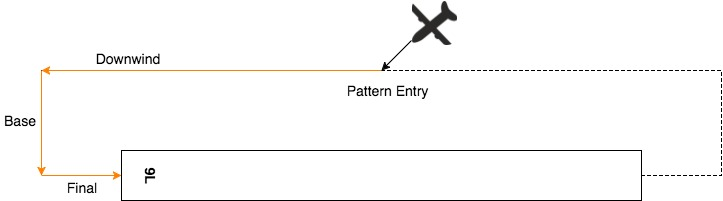
\includegraphics[width=\linewidth]{img/airport_traffic_pattern}
            \caption{Example showing an airport's traffic pattern and the subphases of the approach.}
            \label{fig:traffic_pattern}
        \end{figure}
        
        Along with detecting the approach phase (\Cref{alg:detect_approach}), this section also details the algorithms for detecting \textit{(i)} the airport and runway that the aircraft is approaching and \textit{(ii)} the final turn so it can later be analyzed for an undershoot or overshoot.
        
        The algorithm for detecting an aircraft's approach needs to iterate through all of the time values since there can be multiple approaches within a single flight.  Once the algorithm detects the aircraft is 1 mile away from an airport and is less than 500 feet above ground level (AGL) (\Cref{alg:detect_approach} Line 6), it is determined that the pilot is beginning an approach and a unique approach identifier is generated in order to store metadata later in the process.  Next, the algorithm continues to iterate through time values until either the aircraft goes under 200 ft AGL, or it goes back above 500 ft AGL, which will then be recorded as a go-around later in the process (\Cref{alg:detect_approach} Lines 8-12).  If the aircraft goes under 200 ft AGL, then it is determined to be on the final approach.  The aircraft is considered to be on the final approach while it is within 1 mile away from the airport and it is between 50 and 200 feet AGL inclusive (\Cref{alg:detect_approach} Lines 16-22).
    
    Once the aircraft either goes above 200 feet AGL or goes below 50 feet AGL, then the final approach is marked as finished, and the critical metadata associated with the approach is stored.  At this point, the runway that is being approached can be detected using a combination of the aircraft's current geolocation and heading since the intended runway may not be closest to the aircraft depending on the degree of the final turn (\Cref{alg:detect_approach} Line 24).
        
        %%%%% Detect Approaches Pseudo-code
        \begin{algorithm}
            \begin{algorithmic}[1]\raggedright
            	\State $ \var{airplanePoint} \gets \var{data[i].geoPoint} $
            	\State $ \var{airport} \gets \var{detectAirport(airplanePoint)} $
                \State $ \var{airplaneAltitude} \gets \var{data[i].altitude} $
                \State $ \var{heightAGL} \gets \var{airplaneAltitude} - \var{airport.altitude} $
                \State $ \var{distance} \gets \var{airplanePoint.distanceTo(airport.geoPoint)} $
                \If{$ \var{distance} < 1$\,mi and $\var{heightAGL} < 500$\,ft}
                    \State $ \var{apprID} \gets \var{genNewApproachID()} $
                    \While{$ 200\,\text{ft} < \var{heightAGL} < 500\,\text{ft} $ and $ \var{i} < \var{data.length} $}
                        \State $ \var{airplaneAltitude} \gets \var{data[i].altitude} $
                        \State \var{heightAGL} $ \gets $ \var{airplaneAltitude} $-$ \var{airport.altitude}
                        \State $ i \gets i + 1 $
                    \EndWhile

                    \State $ \var{approachStartTime} \gets i $
                    \State $ \var{airplaneHdg} \gets \var{data[i].hdg} $
                    \State $ \var{airplanePoint} \gets \var{data[i].geoPoint} $

                    \While{$ \var{distance} < 1$\,mi and $ 50\,\text{ft} \leq \var{heightAGL} \leq 200\,\text{ft} $ and $ \var{i} < \var{data.length} $}
                        \State $ \var{airplaneAltitude} \gets \var{data[i].altitude} $
                        \State $ \var{airplanePoint} \gets \var{data[i].geoPoint} $
                        \State $ \var{distance} \gets \var{airplanePoint.distanceTo(airport.geoPoint)} $
                        \State $ \var{heightAGL} \gets \var{airplaneAltitude} - \var{airport.altitude} $
                        \State $ i \gets i + 1 $
                    \EndWhile

                    \State $ \var{approachEndTime} \gets i $
                    \State $ \var{runway} \gets $ \var{detectRunway(airplanePoint, airplaneHdg, airport)}
                    \State \var{approaches[apprID]} $ \gets $ store approach metadata
                    \State \Return \var{(approachStartTime, approachEndTime)}
                \EndIf
            \end{algorithmic}
            \caption{Pseudo-code for function which detects when an aircraft is approaching a runway.}
            \label{alg:detect_approach}
        \end{algorithm}
        
        
        %----------
        % AIRPORT DETECTION
        %----------
        \subsubsection{Airport detection.} \label{sec:detect_airport}
        
        	For identifying the airport that is being approached, a QuadTree~\cite{finkel1974quad} data structure was used.  It was used due to the fact that a two-dimensional tree structure is needed in order to efficiently find the closest airport latitude and longitude point when given the aircraft's latitude and longitude.  The QuadTree is constructed using a list of airport objects from a database then is optimized.  Both the insertion and searching algorithms yield $\mathcal{O}(\log n)$ complexity.


        %----------
        % RUNWAY DETECTION
        %----------
        \subsubsection{Runway detection.}
        
            The algorithm used for finding the runway that is being approached is a simple sequential search with a constraint that the difference between the aircraft's heading and the runway's heading must be within an upper limit.  The reasoning for this constraint is the fact that the runway closest to the aircraft may not necessarily be the one it is approaching depending on the arrangement of the runways and the degree of the final turn (see \Cref{fig:runway_selection}).  A value of $20^\circ$ was used for the heading constraint since it is double the value used for detecting a heading exceedance (see \Cref{tab:approach_thresholds}).  Thus if the runway returned by the algorithm is not the intended runway, it means the aircraft's heading is significantly off-center from the runway's heading and the pilot will need to perform severe corrections to get back on course.
            
            In this case, using a sequential search is efficient enough since an airport has a very small number of runways, whereas there are thousands of airports within the United States which requires a more sophisticated algorithm.  The runway detection algorithm is given in \Cref{alg:detect_runway}.
            
            
            \begin{figure}
            	\centering
				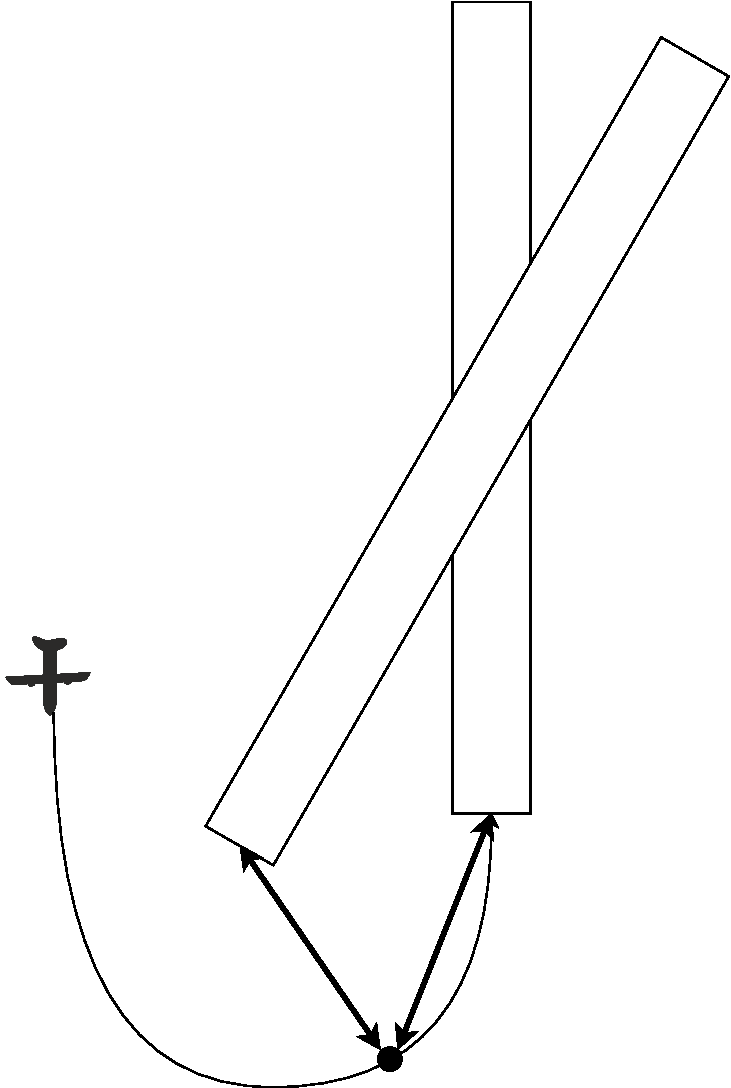
\includegraphics[width=0.5\linewidth]{runway_selection_example}
				\caption{Example showing that the closest runway to the aircraft may not necessarily be the one they are attempting to land on.  If we use the black dot as a reference point for when we attempt to detect the runway, it can be seen that the runway on the left may actually be closer.  However, the aircraft's heading will match closer to the runway on the right (the pilot's intended target).  This is the purpose of searching for the closest runway with a constraint on the heading difference.}
				\label{fig:runway_selection}
            \end{figure}
            

            %%%%% Detect Runway Pseudo-code
            \begin{algorithm}
                \begin{algorithmic}[1]\raggedright
                    \Function{DetectRunway}{airplanePoint, airplaneHdg, airport}
                        \State $ \var{theRunway} \gets \textit{NULL} $
                        \State $ \var{closestDistance} \gets \infty $

                        \For{\var{runway} in \var{airport.runways}}
                            \If{$ \abs{\var{headingDifference(runway.hdg, airplaneHdg)}} \leq 20^\circ $}
                                \State $ \var{distance} \gets \var{airplanePoint.distanceTo(runway.geoPoint)} $
                                \If{$ \var{distance} \le \var{closestDistance} $}
                                    \State $ \var{theRunway} \gets \var{runway} $
                                    \State $ \var{closestDifference} \gets \var{difference} $
                                \EndIf
                            \EndIf
                        \EndFor

                        \State \Return{theRunway}
                    \EndFunction
                \end{algorithmic}
                \caption{Pseudo-code for \textit{detectRunway} function which detects the runway an aircraft is approaching.}
                \label{alg:detect_runway}
            \end{algorithm}
        
        
        %----------
        % FINAL TURN DETECTION
        %----------
        \subsubsection{Final turn detection.}
        
        	In order to detect the final turn subphase of the approach, we first get the previous three minutes of data before the approach ends.  The previous three minutes are used to reduce the search space and because it does not make logical sense for a final turn to occur greater than three minutes before the approach ends.  Next, the algorithm searches for the final turn start and end time.  It finds these by searching for the points at which the aircraft's heading creates a $90^\circ$ and $15^\circ$ angle, respectively, to the runway's heading.  A visualization of these reference points can be seen in \Cref{fig:final_turn_example}.  The search is performed backwards through the slice of data in order to obtain the last occurrence of each angle difference.  Once both points have been found, they are stored for later use in the analysis stage.  If the aircraft did not have a heading difference greater than $90^\circ$ in the final three minutes, the pilot performed a straight-in approach and, consequently, did not execute the final turn subphase.
        	The final turn detection algorithm is given in \Cref{fig:detect_final_turn}.
            
            \begin{figure}
            	\centering
                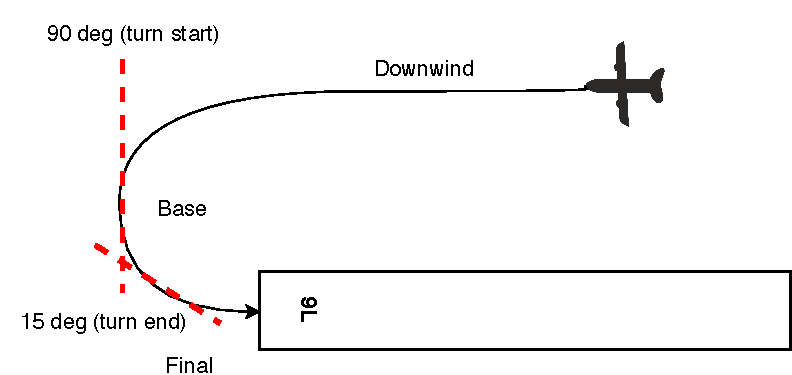
\includegraphics[width=\linewidth]{turn_to_final}
                \caption{Example showing the approach subphases and the slice of data used in the final turn analysis.  The dashed lines represent when the final turn starts ($90^\circ$ heading difference) and ends ($15^\circ$ heading difference).}
                \label{fig:final_turn_example}
            \end{figure}
        
            %%%%% Detect Final Turn Pseudo-code
            \begin{algorithm}
                \begin{algorithmic}[1]\raggedright
                    \Function{DetectFinalTurn}{approachEndTime, runway}
                        \State $ \var{last3Mins} \gets $ get previous 3 mins of data before \var{approachEndTime}
                        \State $ \var{turnStartTime} \gets \textit{NULL} $
                        \State $ \var{turnStartFound} \gets \textit{false} $
                        \State $ \var{turnEndTime} \gets \textit{NULL} $
                        \State $ \var{turnEndFound} \gets \textit{false} $
                        \State $ \var{i} \gets \var{last3Mins.length} - 1 $
                        
                        \Comment Loop backwards through the last 3 mins of data
                        \While{not \var{turnStartFound} and not \var{turnEndFound} and $\var{i} \geq 0$}
                        	\State $ \var{headingError} \gets \abs{\var{headingDifference(runway.hdg, last3Mins[i].hdg)}} $
                            \If{$\var{headingError} \geq 90$ and not \var{turnStartFound}}
                            	\State $ \var{turnStartTime} \gets \var{i} $
                                \State $ \var{turnStartFound} \gets \textit{true} $
                            \EndIf
                            \If{$\var{headingError} \geq 15$ and not \var{turnEndFound}}
                            	\State $ \var{turnEndTime} \gets \var{i} $
                                \State $ \var{turnEndFound} \gets \textit{true} $
                            \EndIf
                            
                            \State $ \var{i} \gets \var{i} - 1 $
                        \EndWhile
                        
                        \State $ \var{approaches[apprID]} \gets $ store final turn metadata
                        \State \Return \var{(turnStartTime, turnEndTime)}
                    \EndFunction
                \end{algorithmic}
                \caption{Pseudo-code for function which detects the final turn subphase of the approach.}
                \label{fig:detect_final_turn}
            \end{algorithm}
        
        
    
    %----------
    % LANDING
    %----------
    \subsection{Landing}
    
    The landing phase is defined as the time from the beginning of the landing flare until the aircraft performs one of the following actions: \textit{(i)} exits the landing runway, \textit{(ii)} comes to a complete stop on the runway (full-stop), or \textit{(iii)} when power is applied for takeoff in the case of a touch-and-go landing~\cite{cictt2013phase}.
    
    The landing phase and result detection is able to differentiate between a full-stop, touch-and-go, and a go-around\footnote{Go-around is included here as a possibility for the result of a landing phase since only one of the full-stop, touch-and-go, and go-around maneuvers can be executed after an approach/landing even though the aircraft does not physically contact the ground.}.  Pseudo-code for this process is given in \Cref{alg:detect_landing}.
    
    This detection algorithm iterates through time values starting where the final approach detection finished (\Cref{alg:detect_landing} Lines 10-29).  It continues to iterate while the aircraft is below 500 feet AGL; or if it is the aircraft's final landing and the time values run out, then it stops analyzing.  While the algorithm iterates through the time values, it checks if the aircraft's indicated airspeed (IAS) is less than or equal to 35 knots (\Cref{alg:detect_landing} Line 13).  If this is true, then it is determined the aircraft is no longer traveling at a flying speed, thus it is making a complete stop.  The stall speed of a Cessna 172S aircraft is 40 knots IAS (KIAS)~\cite{und_poh}; therefore, the value of 35 knots guarantees the aircraft cannot be flying.  In order to detect a touch-and-go landing, the previous five elevation readings are stored and their average is calculated (\Cref{alg:detect_landing} Lines 20-28).  If it is found the aircraft is not making a stop-and-go landing, then the average elevation for the last five seconds is checked to see if it is less than five feet AGL (\Cref{alg:detect_landing} Line 15).  This means the aircraft is still at a flying speed (above 35 knots) and is also maintaining a stable elevation of five feet or less for at least five seconds.
    
    Once the aircraft goes above 500 feet AGL or the time values run out, then the landing result is determined from the conditions found during the analysis (\Cref{alg:detect_landing} Line 32 and \Cref{alg:landing_result_helper}).  If it was found the aircraft was making a complete stop, then a value of ``full-stop'' is stored.  If it was not making a complete stop and had a relatively stable elevation of 5 feet or less above the runway, then a value of ``touch-and-go'' is stored.  The final result type, ``go-around'', is used as a fall-through since there are only three classifications, as mentioned previously.  The three landing result types and how they are detected are summarized in \Cref{tab:landing_types}.
    
    After the landing is classified, then it is determined whether there is a takeoff phase that follows the current landing phase.  If the end of the data has been reached or a go-around is being performed (\Cref{alg:detect_landing} Line 33), there will not be a subsequent takeoff phase.  Otherwise, we need to find the transition from landing to takeoff.  This is done by finding the index of the engine's minimum RPM value between \textit{landingStartTime} and \textit{landingEndTime} (\Cref{alg:detect_landing} Line 36 and \Cref{alg:last_rpm_helper}).  By using the engine's minimum RPM value, we know all RPM values afterwards will be greater, which means the pilot will be using more throttle in order to takeoff.  The \textit{landingEndTime} is then reset to this transition mark.  Lastly, the critical metadata found during the analysis is stored.
    
    %%%%% Detect Landing Pseudo-code
   	\begin{algorithm}
    	\begin{algorithmic}[1]
        \Function{DetectLanding}{approachEndTime, runway}
        	\State $ \var{landingStartTime} \gets \var{approachEndTime} $
        	\State $ \var{i} \gets \var{approachEndTime} $
        	\State $ \var{airplaneAltitude} \gets \var{data[i].altitude} $
            \State $ \var{heightAGL} \gets \var{airplaneAltitude} - \var{runway.altitude} $
            
            \State $ \var{isFullStop} \gets \textit{false} $
            \State $ \var{isTouchAndGo} \gets \textit{false} $
            \State $ \var{elevations} \gets \var{[]}$
            \State $ \var{avg5SecElevation} \gets 5\,\text{ft} + 1 $
            	\Comment value to guarantee first check passes
            
            \While{$\var{heightAGL} < 500$\,ft and $\var{i} < \var{data.length}$}
            	\If{not \var{isFullStop}}
                	\State $ \var{airplaneIAS} \gets \var{data[i].ias} $
                    \If{$ \var{airplaneIAS} \leq 35$\,kts}
                    	\State $ \var{isFullStop} \gets \textit{true} $
                    \ElsIf{$ \var{avg5SecElevation} \leq 5$\,ft}
                    	\State $ \var{isTouchAndGo} \gets \textit{true} $
                    \EndIf
                \EndIf
                \State $ i \gets i + 1 $
                \State $ \var{airplaneAltitude} \gets \var{data[i].altitude} $
                \State $ \var{heightAGL} \gets \var{airplaneAltitude} - \var{runway.altitude} $
                \If{$ \var{elevations.length} < 5$\,seconds}
                	\State $ \var{elevations.append(heightAGL)} $
                \Else
                	\State $ \var{elevations.pop()} $
                    \State $ \var{elevations.append(heightAGL)} $
                    \State $ \var{avg5SecElevation} \gets \var{avg(elevations)} $
                \EndIf
            \EndWhile
            
            \State $ \var{landingEndTime} \gets \var{i} $
            \State $ \var{isEndOfData} \gets \var{landingEndTime} == \var{data.length} - 1 $
            
            \State $ \var{landingResult} \gets \var{getLandingResult(isFullStop, isTouchAndGo)} $
         
            \State $ \var{isFollowedByTakeoff} \gets not (\var{isEndOfData} $ or $ \var{landingType} == \text{`go-around'}) $
            
            \Comment{If landing is followed by a takeoff, then we need to find the transition from landing to takeoff}
            \If{\var{isFollowedByTakeoff}}
            	\State $ \var{landingDataSlice} \gets $ get slice of data between \var{landingStartTime} and \var{landingEndTime}
                
                \Comment{Marks where the pilot is transitioning from landing to takeoff}
            	\State $ \var{lastOccurrence} \gets \var{getLastOccurrenceOfMinRPM(landingDataSlice)} $
                \State $ \var{landingEndTime} \gets \var{lastOccurrence} $
            \EndIf
            
            \State $ \var{approaches[apprID]} \gets $ store landing metadata
            \State \Return \var{(landingStartTime, landingEndTime)}
        \EndFunction
        \end{algorithmic}
        \caption{Pseudo-code for function which detects the landing from its associated approach.}
        \label{alg:detect_landing}
    \end{algorithm}
    
    
    \begin{algorithm}
    	\begin{algorithmic}[1]
        	\Function{GetLandingResult}{isFullStop, isTouchAndGo}
        		\If{\var{isFullStop}}
                    \State $ \var{landingResult} \gets $ `full-stop'
                \ElsIf{\var{isTouchAndGo}}
                    \State $ \var{landingResult} \gets $ `touch-and-go'
                \Else
                    \State $ \var{landingResult} \gets $ `go-around'
                \EndIf
                \State \Return \var{landingResult}
            \EndFunction
        \end{algorithmic}
        \caption{Pseudo-code for \var{getLandingResult} helper function.}
        \label{alg:landing_result_helper}
    \end{algorithm}
    
    
    \begin{algorithm}
    	\begin{algorithmic}[1]
        	\Function{GetLastOccurrenceOfMinRPM}{dataSlice}
        		\State $ \var{minRPM} \gets \var{min(dataSlice[`rpm'])} $
                \State $ \var{lastOccurrence} \gets 0 $
                \State $ \var{i} \gets 0 $
                
                \While{$\var{i} < \var{dataSlice.length}$} \Comment{loop through slice of data to find last occurrence of minimum RPM}
                	\If{\var{dataSlice[i].rpm} == \var{minRPM}}
						\State $ \var{lastOccurrence} \gets \var{i} $
                    \EndIf
                \EndWhile
                \State \Return \var{lastOccurrence}
            \EndFunction
        \end{algorithmic}
        \caption{Pseudo-code for \var{getLastOccurrenceOfMinRPM} helper function.}
        \label{alg:last_rpm_helper}
    \end{algorithm}
    
    %%%%% Landing Types Table
    \begin{table}
        \caption{\small{Landing result types and their conditions.}}
        \label{tab:landing_types}
        \vspace{3pt}
        \centering
        \begin{tabular}{@{} c m{.70\linewidth} @{}}
            \hline
            \bfseries Type & \bfseries Condition \\ \hline
            full-stop    & Aircraft's indicated airspeed speed (IAS) falls below 35 knots \\ \hline
            touch-and-go & Aircraft is not making a complete stop and maintains a stable altitude of five feet AGL or less for at least five seconds \\ \hline
            go-around    & All other cases \\ \hline
        \end{tabular}
    \end{table}
    

%----------------------------------------
% PHASE QUALITY ANALYSIS
%----------------------------------------
\section{Phase of Flight Quality Analysis \& Exceedance Detection} \label{sec:phase_quality}
    
    %----------
    % APPROACH
    %----------
	\subsection{Approach}
        
        Along with analyzing the approach phase, this section also details the algorithms for analyzing \textit{(i)} the final turn subphase for an undershoot or overshoot and \textit{(ii)} the pilot's self-defined glide path angle.
        
        The algorithm for analyzing an approach phase iterates through all the time values found during the phase identification stage (\Cref{alg:analyze_approach} Lines 4-17).  For each time value, the analysis for unstableness is performed.  During this analysis, several flight parameters are checked against predetermined thresholds to see if any were exceeded (\Cref{alg:analyze_approach} Lines 8-11).  The values used for the thresholds are summarized in \Cref{tab:approach_thresholds}.  A \textit{true} value for a condition means the parameter is stable.  Thus, if any of the parameters are unstable, \var{isUnstable} will result to being \textit{true}, meaning the entire aircraft is in an unstable state (\Cref{alg:analyze_approach} Line 12).  If the aircraft is found to be unstable, the corresponding time value is stored as well as the parameter values that caused the unstableness (\Cref{alg:analyze_approach} Line 14).
        
        %%%%% Exceedance Thresholds Table
        \begin{table}
            \caption{\small{Stabilized approach criteria for Cessna 172S~\cite{und_flight_manual}.}} \label{tab:approach_thresholds}
            \vspace{3pt}
            \centering
            \begin{tabular}{@{} c >{\raggedright\arraybackslash} m{.3\linewidth} m{.42\linewidth} @{}}
                \hline\noalign{\smallskip}
                \bfseries Parameter & \bfseries Description & \bfseries Value \\
                \noalign{\smallskip}
                \hline
                \noalign{\smallskip}
                F & Flight path correct & Less than 10$^\circ$ off runway heading, less than 50 ft left or right of the runway center line (cross track error) \\ \hline
                L & Landing configuration correct & N.A. \\ \hline
                A & Airspeed proper & Indicated airspeed (IAS) within 55-75 kts \\ \hline
                P & Power setting appropriate & N.A. \\ \hline
                S & Sink rate appropriate & Vertical speed indicated (VSI) does not exceed -1000 ft/min \\ \hline
            \end{tabular}
        \end{table}
        
        
        %%%%% Analyze Approach Pseudo-code
        \begin{algorithm}
            \begin{algorithmic}[1]\raggedright
            \Function{AnalyzeApproach}{startTime, endTime, runway}
                \State $ \var{approachDataSlice} \gets $ get slice of data between \var{startTime} and \var{endTime}
                \State $ \var{i} \gets 0 $
                \While{$\var{i} < \var{approachDataSlice.length}$}
                    \State $ \var{airplaneHdg} \gets \var{approachDataSlice[i].hdg} $
                    \State $ \var{airplaneIAS} \gets \var{approachDataSlice[i].ias} $
                    \State $ \var{airplaneVSI} \gets \var{approachDataSlice[i].vsi} $
                    \State $ \var{airplanePoint} \gets \var{approachDataSlice[i].geoPoint} $

                    \State $ \var{headingIsStable} \gets 180^\circ - \abs{\abs{\var{runway.hdg} - airplaneHdg} - 180^\circ} \leq 20^\circ $
                    \State $ \var{crossTrackIsStable} \gets \var{calculateCrossTrack(} \break \var{airplanePoint, airplaneHdg, runway)} \leq 50\,\text{ft} $
                    \State $ \var{iasIsStable} \gets 55\,\text{kts} \leq \var{airplaneIAS} \leq 75\,\text{kts} $
                    \State $ \var{vsiIsStable} \gets \var{airplaneVSI} \geq -1000\,\text{ft/min} $
                    \State $ \var{isUnstable} \gets $ not (\var{headingIsStable} and \var{crossTrackIsStable} and \var{iasIsStable} and \var{vsiIsStable})

                    \If{\var{isUnstable}}
                        \State $ \var{approaches[apprID]} \gets $ store index as unstable and corresponding unstable parameter values
                    \EndIf

                    \State $ \var{i} \gets \var{i} + 1 $
                \EndWhile
            \EndFunction
            \end{algorithmic}
            \caption{Pseudo-code for function which analyzes an approach for unstableness.}
            \label{alg:analyze_approach}
        \end{algorithm}
        
        
        %----------
        % Final Turn
        %----------
        \subsubsection{Final turn.}
        
        	The final turn subphase is very critical for achieving a flight path aligned with the runway.  Since the end of the turn occurs fairly late in the approach phase, any mistakes can greatly reduce the pilot's ability to stabilize the aircraft by 200 ft AGL.  If the pilot makes a turn that is too sharp (undershoot) or too wide (overshoot), they may have to make a large corrective maneuver to re-align themselves, which could stall the aircraft if performed incorrectly and potentially result in a loss of control (LOC) event.  Stalls and loss of control events contributed to 52.0\% and 17.4\% of all landing accidents in 2014~\cite{kenny201726th}, respectively. 
            
            Analyzing this subphase only requires the end time value and runway found during the identification stage.  For this single time value, the aircraft's cross track error is calculated (\Cref{alg:analyze_final_turn} Line 5).  Next, the direction of the turn is determined by calculating which roll attitude direction was greater\footnote{If the aircraft rolls to the left, it is recorded as a negative degree and vice versa if the aircraft rolls to the right.  This is why we find the minimum roll attitude as the highest degree in which aircraft rolled left, and the maximum roll attitude as the highest degree in which the aircraft rolled right.} (\Cref{alg:analyze_final_turn} Lines 6-12).  The severity of the cross track error is then determined (\Cref{alg:analyze_final_turn} Lines 13-19).  A Risk Level 1 error is a value greater than 25 feet, while a Risk Level 2 error is a value greater than 100 feet.  The turn error is determined next based on the roll direction and direction of the cross track error (\Cref{alg:analyze_final_turn} Lines 20-32).  For example, if the pilot rolled left and had a negative cross track error\footnote{Meaning they are left of the runway's centerline.}, it is considered an ``undershoot''.  See \Cref{tab:final_turn_matrix} for all possible combinations of roll direction and cross track error.  However, if the cross track error is less than a Level 1 risk, then the turn is considered to be safe and a Risk Level 0 is stored (\Cref{alg:analyze_final_turn} Line 18).  Lastly, the turn error and severity are stored.  See \Cref{fig:final_turn_examples} for visualizations of several different final turn scenarios.
            
            If a final turn was not found in the detection phase (due to the pilot performing a straight-in approach), the analysis stage will be skipped.
            
            
            \begin{figure}
            	\centering
                \subfloat[Aligned.\label{fig:aligned_example}]{
                	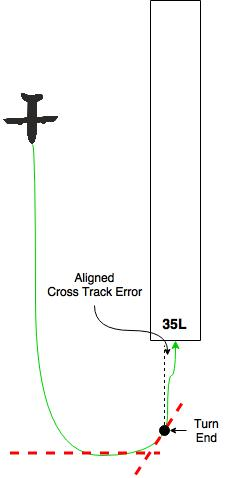
\includegraphics[width=0.29\textwidth]{img/aligned}
                }\hfill%
                \subfloat[Undershoot.  In this case, it is a small severity (Level 1) and color-coded as orange.\label{fig:undershoot_example}]{
                	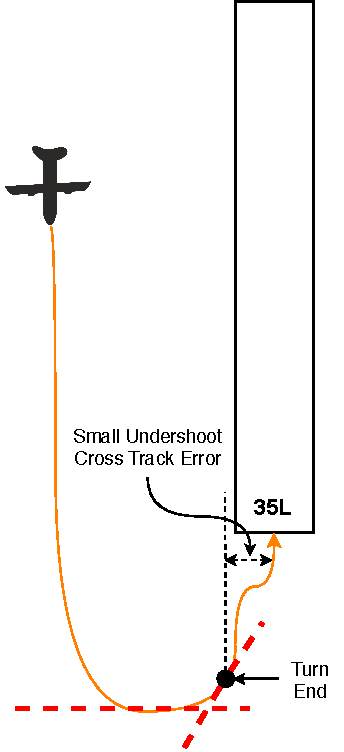
\includegraphics[width=0.29\textwidth]{img/undershoot}
                }\hfill%
                \subfloat[Overshoot.  In this case, it is a large severity (Level 2) and color-coded as red.\label{fig:overshoot_example}]{
                	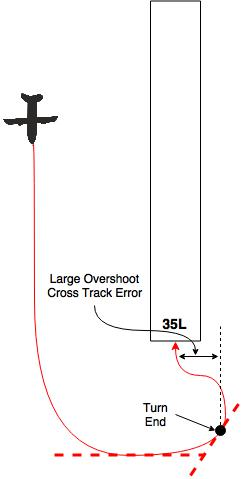
\includegraphics[width=0.29\textwidth]{img/overshoot}
                }%
                \caption{Examples showing various final turn qualities.}
                \label{fig:final_turn_examples}
            \end{figure}
            
            
            \begin{table}
            	\centering
                \caption{\small{Final turn matrix of the combinations of roll direction and cross track error.}} \label{tab:final_turn_matrix}
                \vspace{3pt}
                \begin{tabular}{|>{\bfseries}c | c c|}
                	\hline
                    \bfseries \diagbox{Direction}{Cross Track} & \bfseries $\mathbf{< 0}$\,ft & \bfseries $\mathbf{> 0}$\,ft \\
                    \hline
                    Left  & Undershoot & Overshoot \\ \hline
                    Right & Overshoot  & Undershoot \\ \hline
                \end{tabular}
            \end{table}
            
            
            %%%%% Analyze Final Turn Pseudo-code
            \begin{algorithm}
                \begin{algorithmic}[1]\raggedright
                \Function{AnalyzeFinalTurn}{startTime, endTime, runway}
                    \State $ \var{turnDataSlice} \gets $ get slice of data between \var{startTime} and \var{endTime}
                    \State $ \var{airplaneHdg} \gets \var{turnDataSlice[endTime].hdg} $
                    \State $ \var{airplanePoint} \gets \var{turnDataSlice[endTime].geoPoint} $
                    \State $ \var{crossTrackError} \gets \var{calculateCrossTrack(} \break \var{airplanePoint, airplaneHdg, runway)} $
                    
                    \State $ \var{leftDirection} \gets \abs{\var{min(turnDataSlice[`roll'])}} $
                    \State $ \var{rightDirection} \gets \abs{\var{max(turnDataSlice[`roll'])}} $
                    \If{$\var{leftDirection} > \var{rightDirection}$}
                    	\State $ \var{rollDirection} \gets $ `left'
                    \Else
                    	\State $ \var{rollDirection} \gets $ `right'
                    \EndIf
                    
                    \If{$\abs{\var{crossTrackError}} > 100$\,ft}   \Comment Level 2
                    	\State $ \var{severity} \gets $ 2
                    \ElsIf{$\abs{\var{crossTrackError}} > 25$\,ft} \Comment Level 1
                    	\State $ \var{severity} \gets $ 1
                    \Else
                    	\State $ \var{severity} \gets $ 0
                    \EndIf
                    
                    \If{\var{rollDirection} == `left'}
                        \If{$\var{crossTrackError} < 0$}
                        	\State $ \var{turnError} \gets $ `undershoot'
                        \Else
                        	\State $ \var{turnError} \gets $ `overshoot'
                        \EndIf
                    \Else
                        \If{$\var{crossTrackError} > 0$}
                        	\State $ \var{turnError} \gets $ `undershoot'
                        \Else
                        	\State $ \var{turnError} \gets $ `overshoot'
                        \EndIf
                    \EndIf
                    
                    \State $ \var{approaches[apprID]} \gets $ store severity and error
                    
                    \State \Return \var{(severity, turnError)}
                \EndFunction
                \end{algorithmic}
                \caption{Pseudo-code for function which analyzes the quality of a final turn phase.}
                \label{alg:analyze_final_turn}
            \end{algorithm}
        
        
        %----------
        % SELF-DEFINED GLIDE PATH
        %----------
        \subsubsection{Self-defined glide path.}
        
        	A majority of runways in the U.S. publish an ideal glide slope that all pilot's should adhere to.  However, not all runways have a published glide slope.  Therefore, a method for analyzing the aircraft's actual glide path angle (GPA) during the final approach is needed in order for the pilot to be able to see what their average GPA was and how well they adhered to it.  This is why we termed this method a ``self-defined glide path angle''.  \Cref{fig:self_defined_example} shows an example of what the self-defined glide path analysis is performing.
            
            Major deviations from the ideal glide slope can be very costly.  For example, if the pilot is approaching at a steep angle, a hard landing or a landing short of the runway can occur.  On the other hand, if the pilot is approaching at a shallow angle, a runway overrun can occur.
            
            First, the slice of data for the corresponding approach phase found during the detection stage is obtained (\Cref{alg:analyze_glide_path} Line 2).  Next, a linear regression using the least squares approach is calculated (\Cref{alg:analyze_glide_path} Line 3) using the aircraft's height AGL (dependent variable) over all the time values (independent variable).  From that calculation we obtain the y-intercept, slope, and r-value (correlation coefficient) of the linear regression model (\Cref{alg:analyze_glide_path} Lines 4, 5, 15).  Then, all the necessary values for computing the pilot's defined GPA are calculated (\Cref{alg:analyze_glide_path} Lines 6-13).  Once all the supporting values are found, then the actual GPA is calculated using the $\arctan$ of the predicted vertical distance dropped over the traveled horizontal distance (\Cref{alg:analyze_glide_path} Line 14).  Furthermore, the square of the r-value is calculated (\Cref{alg:analyze_glide_path} Line 16), which explains how well the pilot's glide path ``fit'' the ideal glide path.  Lastly, the calculated values and metadata are stored in the database.
            
            
            \begin{figure}[t]
            	\centering
                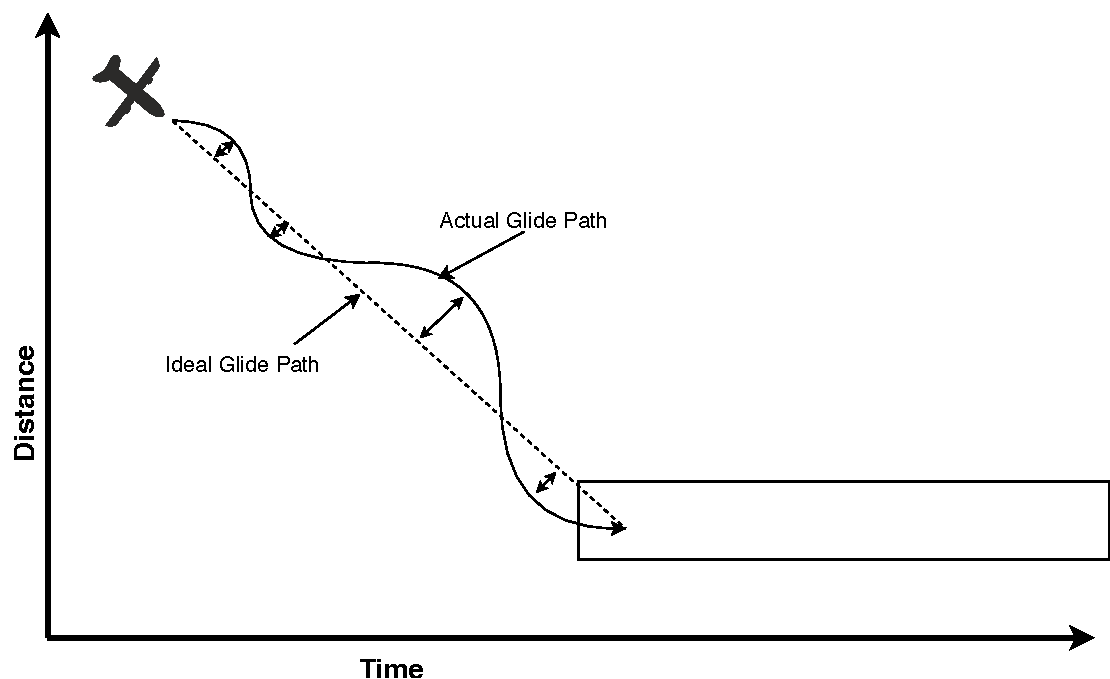
\includegraphics[width=\linewidth]{img/self_defined_example}
                \caption{Example showing the self-defined glide path angle analysis.  This shows a side view of the pilot oscillating about the glide slope during the approach phase.  The calculation uses a linear regression of the aircraft's vertical distance over time fitted using the least squares approach.  The solid line is the aircraft's actual glide path while the dotted line is the ideal glide path.}
                \label{fig:self_defined_example}
            \end{figure}
            
            
            %%%%% Analyze Self-Defined Glide Path Pseudo-code
            \begin{algorithm}[t]
                \begin{algorithmic}[1]\raggedright
                \Function{AnalyzeGlidePath}{startTime, endTime, runway}
                    \State $ \var{approachDataSlice} \gets $ get slice of data between the approach \var{startTime} and \var{endTime}
                    
                    \State $ \var{regressionResult} \gets \var{linearRegression(} \break \var{approachDataSlice[`time'], approachDataSlice[`agl'])} $
                    \State $ \var{yIntercept} \gets \var{regressionResult.intercept} $
                    \State $ \var{slope} \gets \var{regressionResult.slope} $
                    
                    \State $ \var{maxDistance} \gets \var{max(approachDataSlice[`distance'])} $
                    \State $ \var{minDistance} \gets \var{min(approachDataSlice[`distance'])} $
                    \State $ \var{horizontalDistance} \gets \var{maxDistance} - \var{minDistance} $
                    
                    \State $ \var{maxTime} \gets \var{max(approachDataSlice[`time'])} $
                    \State $ \var{minTime} \gets \var{min(approachDataSlice[`time'])} $
                    
                    \State $ \var{predictedMaxAGL} \gets \var{slope} * \var{maxTime} + \var{yIntercept} $
                    \State $ \var{predictedMinAGL} \gets \var{slope} * \var{minTime} + \var{yIntercept} $
                    
                    \State $ \var{predictedVerticalDistance} \gets \var{predictedMaxAGL} - \var{predictedMinAGL} $
                    
                    \State $ \var{actualGlidePathAngle} \gets \var{degrees(} \break \var{atan(predictedVerticalDistance / horizontalDistance))} $
                    
                    \State $ \var{pearsonsR} \gets \var{regressionResult.rvalue} $
                    \State $ \var{rSquared} \gets \var{pearsonsR} * \var{pearsonsR} $
                    
                    \State $ \var{approaches[apprID]} \gets $ store self-defined glide path metadata
                    \State \Return \var{(actualGlidePathAngle, rSquared)}
                \EndFunction
                \end{algorithmic}
                \caption{Pseudo-code for function which analyzes the quality of the aircraft's glide path angle during the approach phase.}
                \label{alg:analyze_glide_path}
            \end{algorithm}
    

%----------------------------------------
% GRADING METRICS
%----------------------------------------
\section{Grading Metrics}
    
    When creating the risk level metrics to be used for grading the approach analysis data, we wanted to ensure they were backed by statistics obtained from the results from the sample set of flights.  Towards that goal, the risk level metrics have been created from the data found during the approach quality analysis.  For each parameter of concern, the recorded values across all approach phases in the sample set were used to create a normalized histogram showing the probability density of each value range.  From these histograms, the mean and standard deviation were calculated in order to create a best-fit line to overlay the histogram.  The charts were then analyzed by an aviation statistics expert at the University of North Dakota who gave his opinion on reasonable values to use for Risk Level 1 and 2 value ranges based on each mean, standard deviation, and best-fit line.  Even though those elements were created from the analysis statistics, the aviation expert wanted to also ensure the safe value ranges (Risk Level 0) did not conflict with the values published in UND's standardization manual~\cite{und_flight_manual} and the Cessna C172S Pilot's Operating Handbook (POH)~\cite{und_poh}.
    
    After the risk level metrics have been established, the approach quality analysis results will be re-processed and graded according to the metrics.  The resulting grade is then stored along with the other generated approach analysis data within the database.  The specific details of the grading results from using the risk level metrics will be discussed further in \Cref{ch:results}.
    
    
%----------------------------------------
% WEB INTERFACES
%----------------------------------------
\section{Web Interfaces}

	This Section details the newly developed web pages for the NGAFID, which dynamically display results based on the user's chosen filters.  At the time of this writing, there have been new tools developed for each of the approach, final turn, and self-defined glide path analyses.  Each tool will be discussed further in the subsequent Subsections.
    
    
    %----------
    % APPROACH
    %----------
    \subsection{Approach}
    
    	A new web page was implemented in the NGAFID for the purpose of dynamically displaying the approach analysis results produced by the \toolname\ to users (\Cref{fig:approach_tool_screenshot}).  The results are given in four tabs, one for each parameter, as histograms over a specified date range.  A user is able to dynamically add additional date ranges, which will create an additional series in the chart for comparison.  This feature can be used to detect changes in trends over time.  A user is also, optionally, able to filter the results to an airport and further filter to a single runway.  This will allow users to identify trends that are potentially occurring at a specific runway but not at any other runways.
    
    	\begin{figure}
    		\centering
            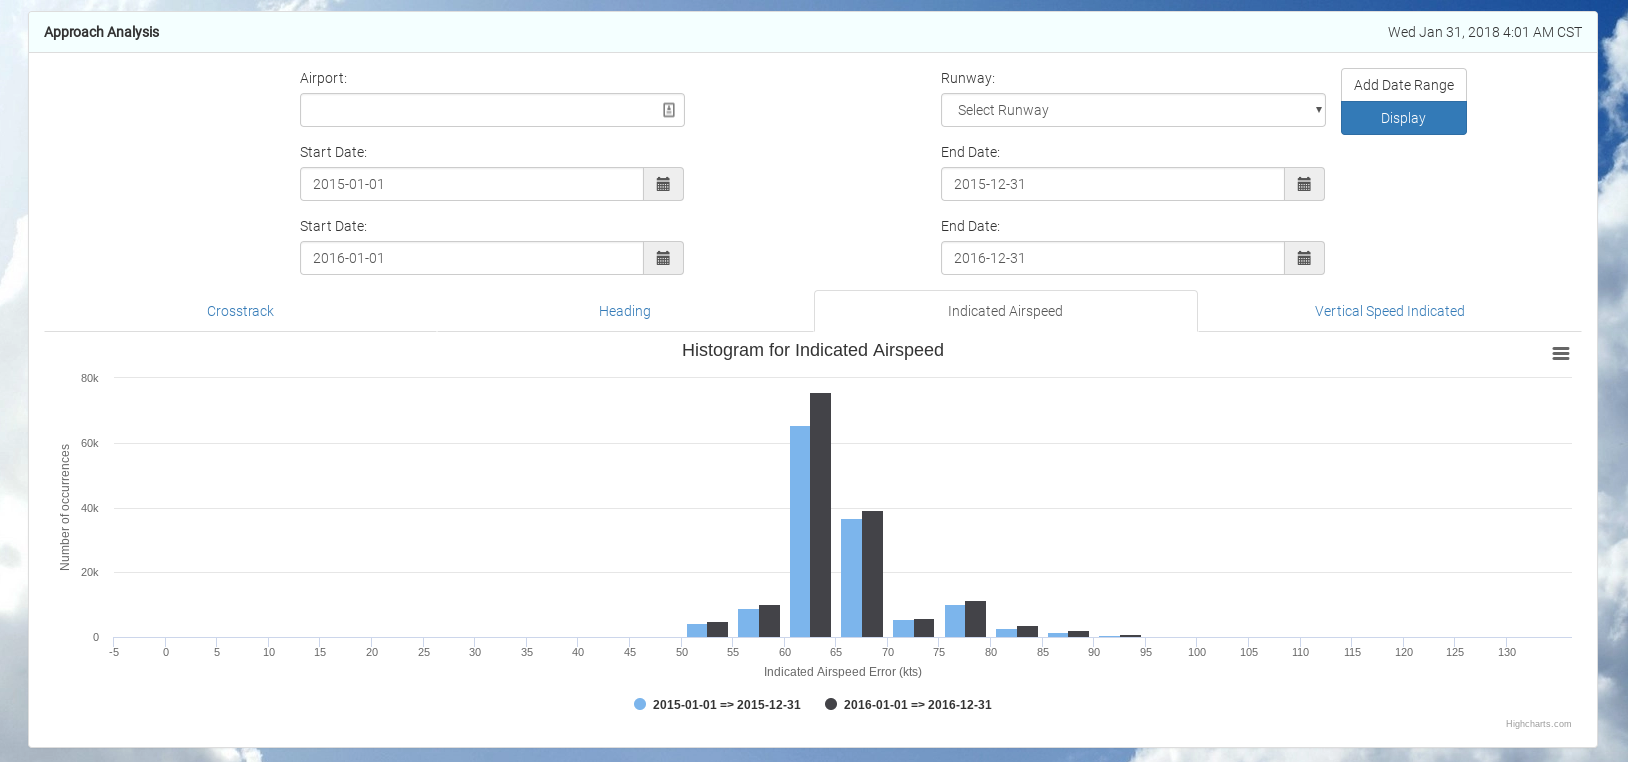
\includegraphics[width=\linewidth]{img/approach_tool_screenshot}
            \caption{A screenshot of the Approach analysis tool on the NGAFID.  It is showing the histogram for indicated airspeed error with two date range filters: 2015-01-01 to 2015-12-31 and 2016-01-01 to 2016-12-31.  The frequency of exceedances can be seen with all values that fall outside of the 55-75 knots range.}
            \label{fig:approach_tool_screenshot}
    	\end{figure}
    
    
    %----------
    % FINAL TURN
    %----------
    \subsection{Final Turn}
    
    	The tool developed for analyzing final turn phases in the NGAFID was implemented with two modes:  \textit{(i)} ``Single Flight'' and \textit{(ii)} ``Aggregate''.
    
    	For the ``Single Flight'' mode, the user can input an ID for a specific flight they'd like to analyze (\Cref{fig:single_ttf_screenshot}).  Once the user clicks the ``Display Single Flight'' button, the interactive map then dynamically transitions to the first approach for that flight.  The map will only display one approach at a time; although, there are tabs across the top for each approach which the user can choose.  Once a different tab is chosen, the map automatically transitions the view to that corresponding approach.  The flight path shows different color codings for the separate final turn, approach, and landing phases as well as different colors for the final turn specifically depending on the severity of the turn error.  A Level 1 turn error will be colored yellow, while a Level 2 turn error will be colored red.  If the turn error is less than the Level 1 criteria, it is colored green.  The user is also able to download a PNG screenshot of the map by clicking the ``Download PNG'' button.
        
        For the ``Aggregate'' mode; the user can choose a specific airport, runway, and month and year combination; which will then display all the approaches that occurred at the chosen runway during the chosen time-frame (\Cref{fig:agg_ttf_screenshot}).  This mode allows a user to see trends in final turn phases during a given time span.  This mode displays the same color code scheme as the ``Single Flight'' mode.
    
    	\begin{figure}
    		\centering
            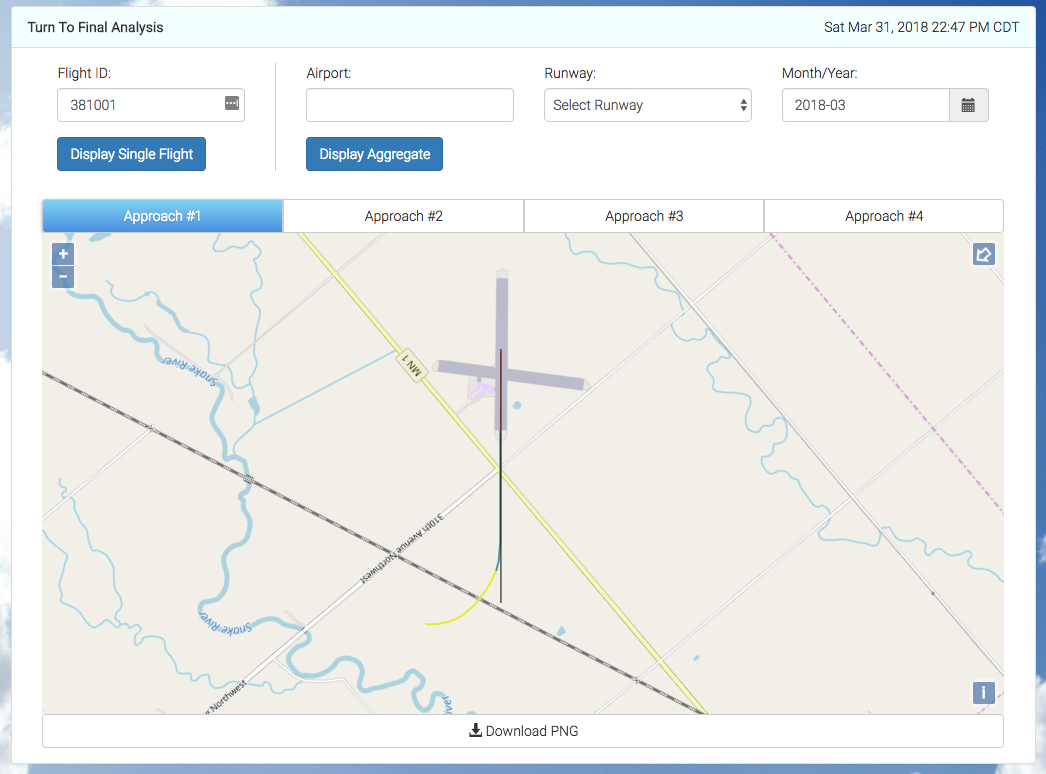
\includegraphics[width=\linewidth]{img/single_ttf_screenshot}
            \caption{A screenshot of the Final Turn analysis tool on the NGAFID in ``Single Flight'' mode.  It is currently showing approach \#1 for Flight ID \#381001.  Approach \#1 shown here had a Level 1 (yellow color code) undershoot.}
            \label{fig:single_ttf_screenshot}
    	\end{figure}
        
        \begin{figure}
    		\centering
            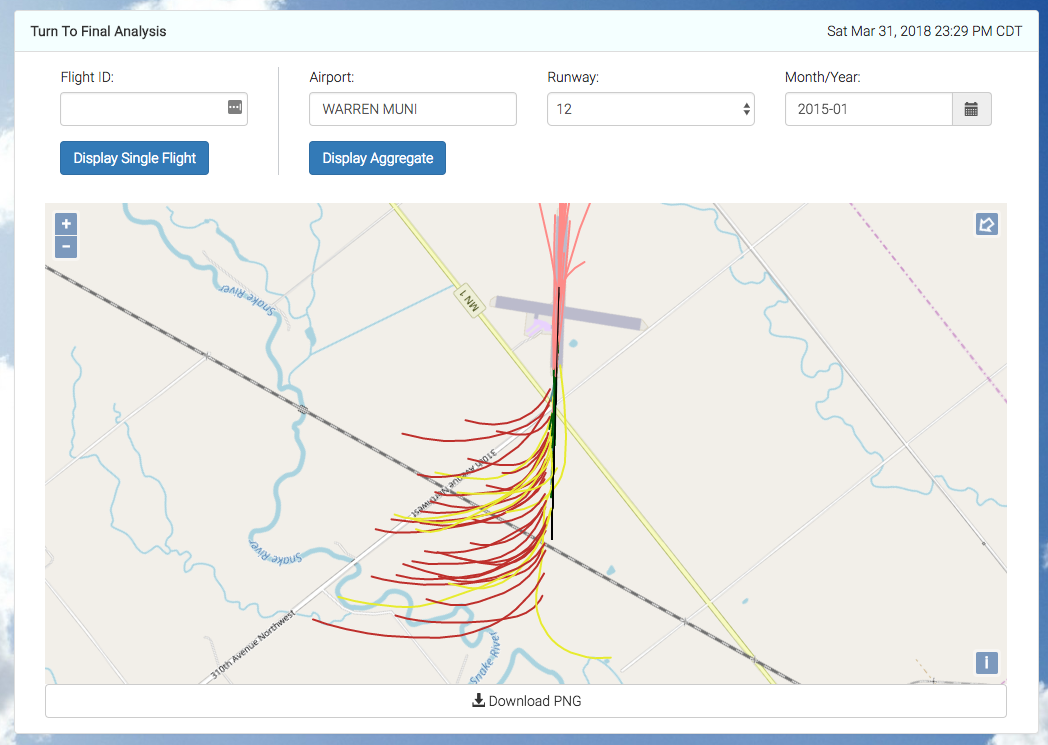
\includegraphics[width=\linewidth]{img/agg_ttf_screenshot}
            \caption{A screenshot of the Final Turn analysis tool on the NGAFID in ``Aggregate'' mode.  It is currently showing all approaches at the Warren Municipal Airport (KD37) for Runway 12 during the month of January 2015.  The many red and yellow lines coming in from the left side mean that a majority of the turns were Level 1 \& 2 undershoots.}
            \label{fig:agg_ttf_screenshot}
    	\end{figure}
    
    %----------
    % SELF-DEFINED
    %----------
    \subsection{Self-Defined Glide Path}
    
    	The tool implemented in the NGAFID for displaying the results of the self-defined glide path analysis currently only supports an aggregate mode (\Cref{fig:self_defined_screenshot}).  It works similarly to the final turn tool as the user chooses an airport, runway, and month and year combination.  This will then display a sideways histogram of all the approaches at the given runway during the given time-frame.  The y-axis shows glide path angles from $0^\circ$ to $10^\circ$ in $0.5^\circ$ increments, and the x-axis shows the number of occurrences that fell within each angle bin.  Lastly, the user can download an image of the displayed chart by clicking the ``hamburger'' menu button.
    
    	\begin{figure}
    		\centering
            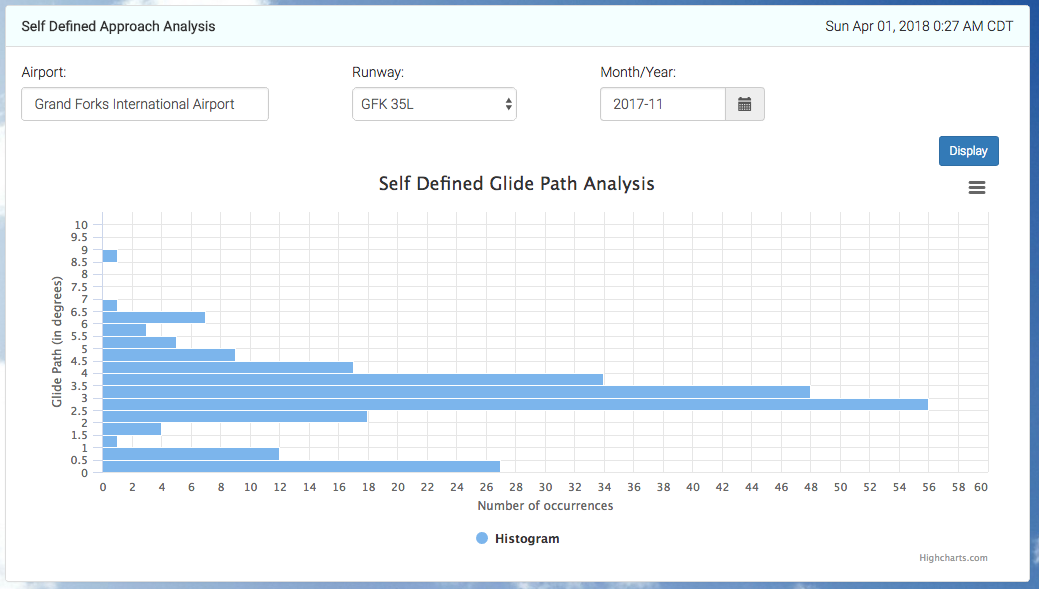
\includegraphics[width=\linewidth]{img/self_defined_screenshot}
            \caption{A screenshot of the Self-Defined Approach analysis tool on the NGAFID.  It is currently showing all approaches at the Grand Forks International Airport (KGFK) for Runway 35L during the month of November 2017.  It displays a sideways histogram with glide path angles on the y-axis and the number of occurrences for each angle on the x-axis.}
            \label{fig:self_defined_screenshot}
    	\end{figure}


